% Tento soubor nahraďte vlastním souborem s přílohami (nadpisy níže jsou pouze pro příklad)

% Pro kompilaci po částech (viz projekt.tex), nutno odkomentovat a upravit
%\documentclass[../projekt.tex]{subfiles}
%\begin{document}

% Umístění obsahu paměťového média do příloh je vhodné konzultovat s vedoucím
%\chapter{Obsah přiloženého paměťového média}

%\chapter{Manuál}

%\chapter{Konfigurační soubor}

%\chapter{RelaxNG Schéma konfiguračního souboru}

%\chapter{Plakát}

\begin{figure}[h!]
	\centering
	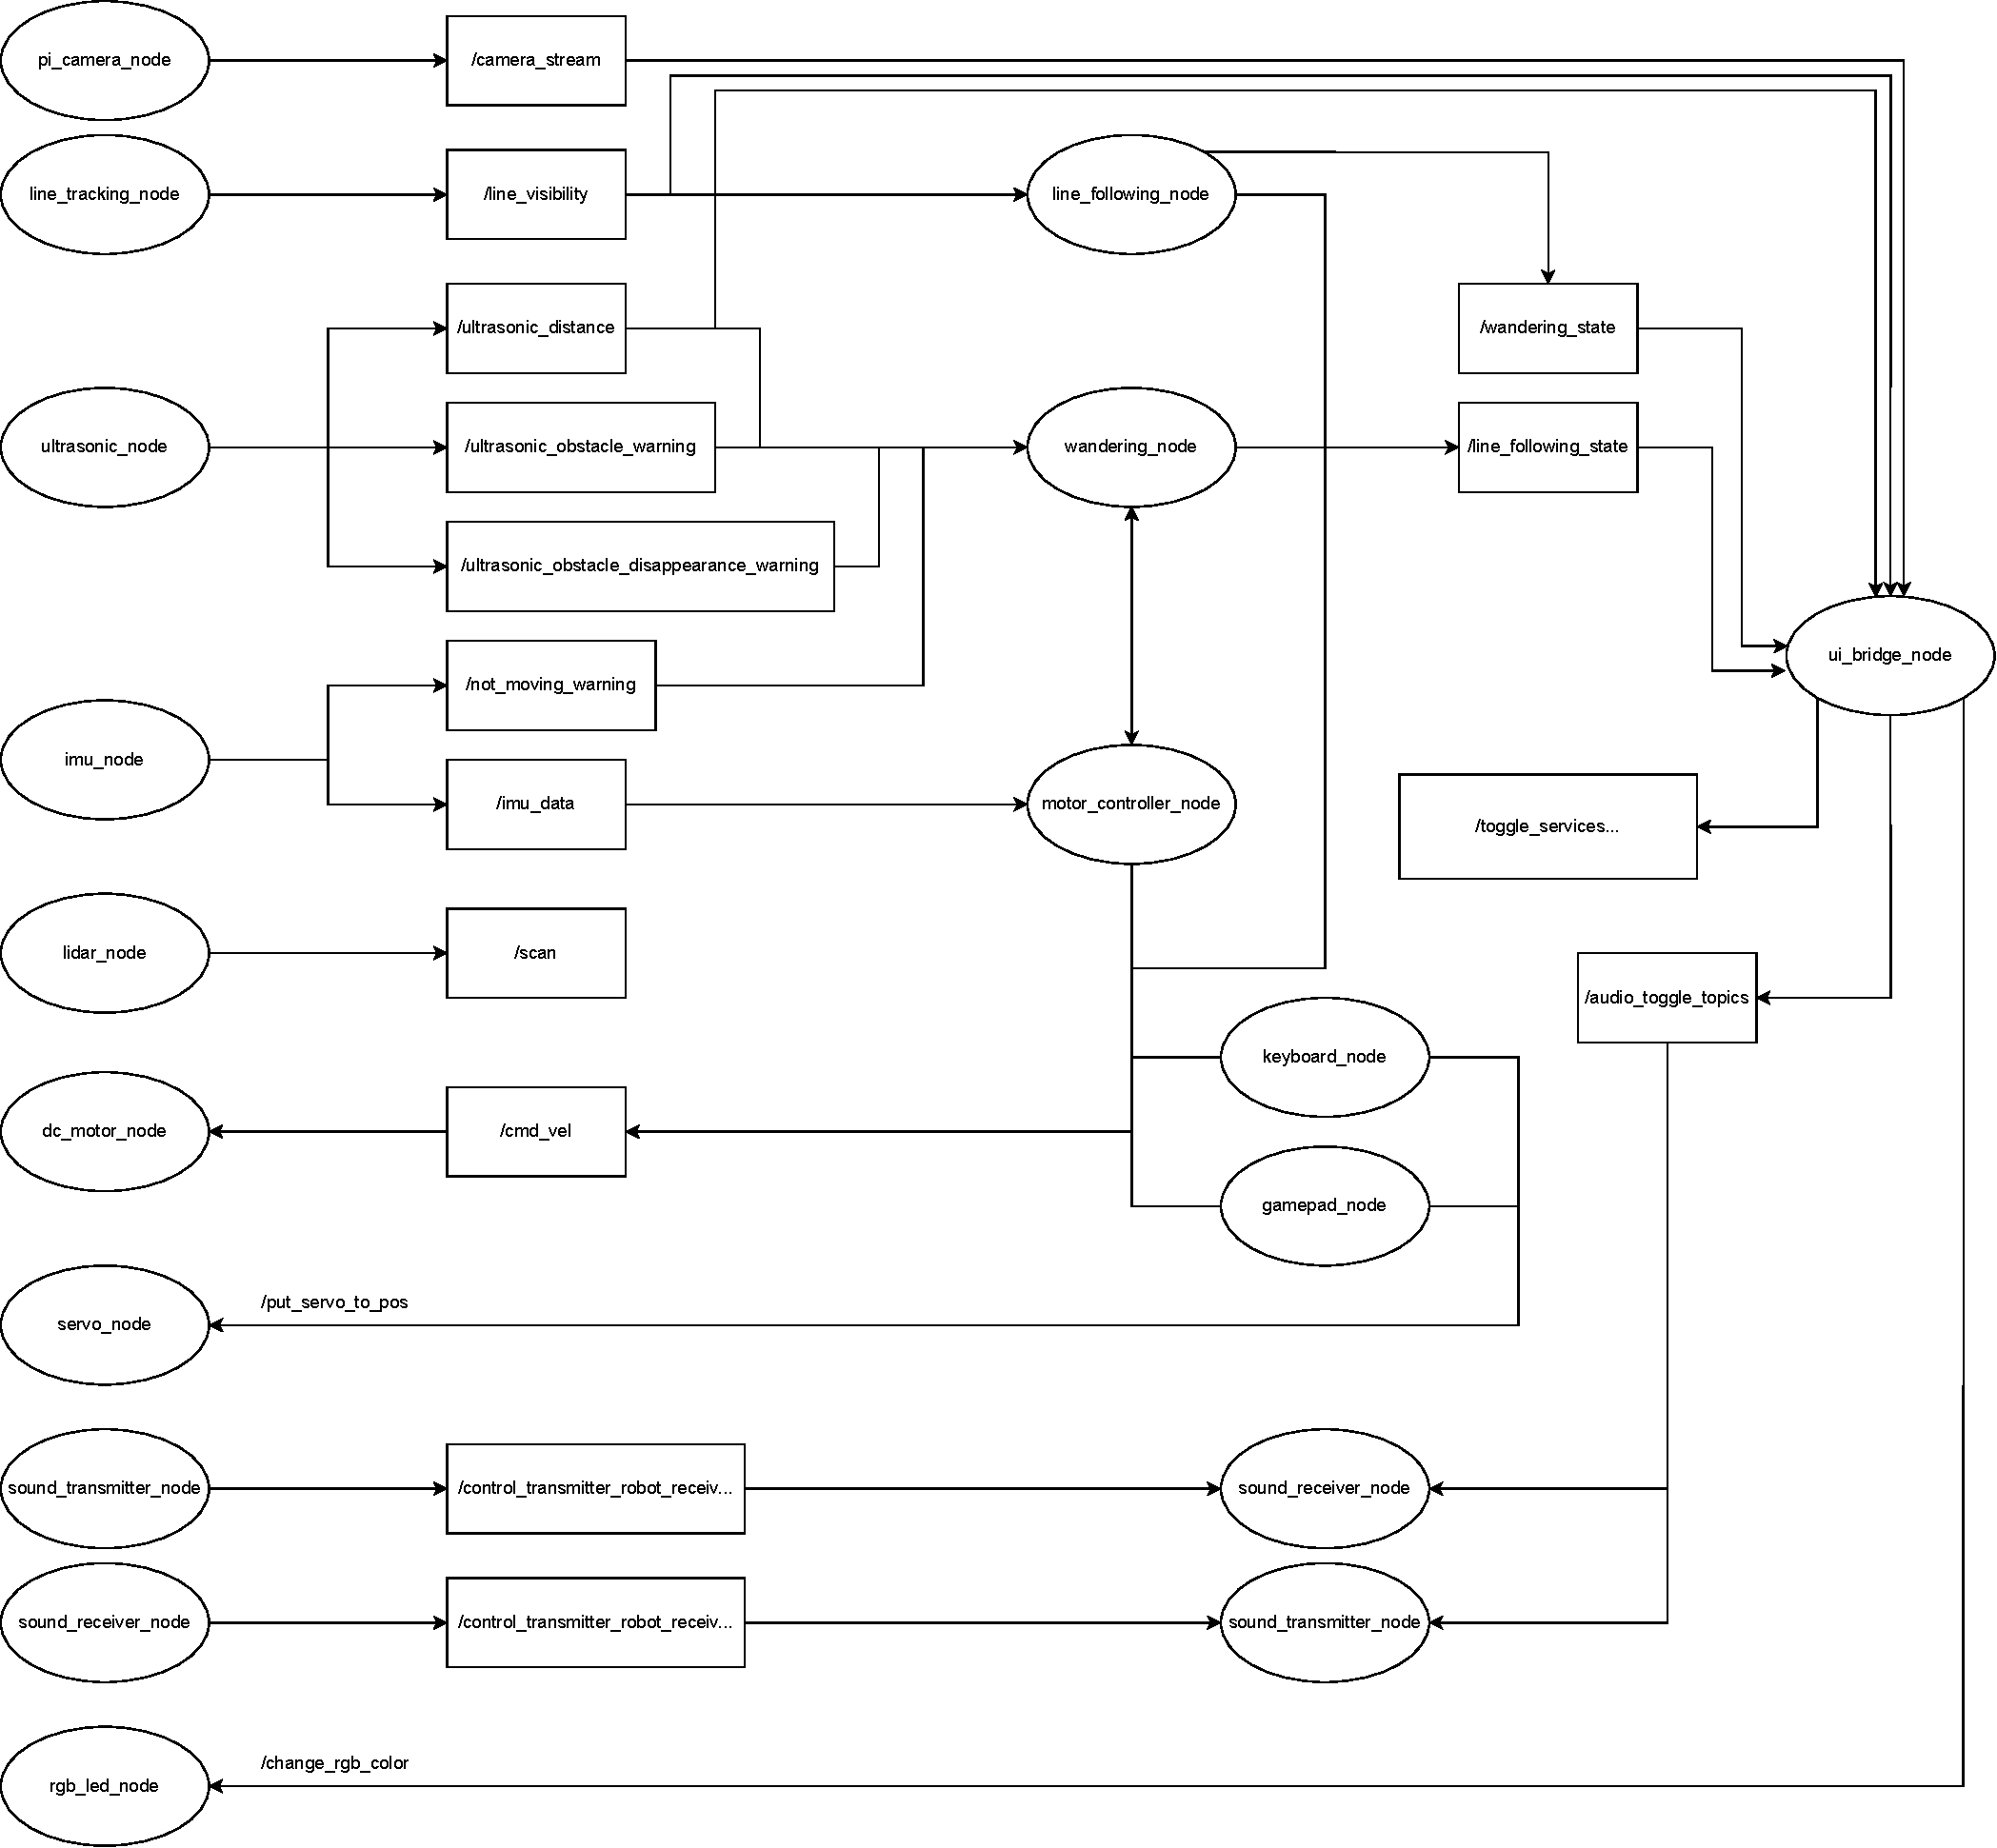
\includegraphics[scale=0.3]{obrazky-figures/ros2_system.pdf}
	\caption{Výsledný ROS2 systém bez slam navigace a gazeba}
	\label{}
\end{figure}

% Pro kompilaci po částech (viz projekt.tex) nutno odkomentovat
%\end{document}
